\documentclass[11pt]{article}
\usepackage[margin=1in]{geometry}
\usepackage{amsmath,amssymb,graphicx,booktabs,xcolor,braket,hyperref}
\usepackage{tikz}
\usepackage{quantikz}   % provides the quantikz environment (quantikz2)
\newcommand{\GCR}{\mathrm{GCR}}
\title{\textbf{BB1(GCR): the ideal pulse, why its physical form fails,\\ and two candidate fixes}}
\author{}
\date{\today}
\begin{document}
\maketitle

\noindent This note collects, in one place, the behaviour of the BB1(GCR) composite pulse used
for GKP modular readout: its \emph{ideal} (non-unitary) form, the reason its physically
realizable (unitary) form fails, and the two fixes we examined --- a deterministic
\emph{pulse-splitting} fix (which does not work) and a probabilistic \emph{heralded} fix (which
does). All numbers are QuTiP simulations at $\Delta=0.34$, $|\alpha|=\sqrt{\pi}/2$, target
$\theta_t=\pi/2$; the readout operating points are $\langle x\rangle\in\sqrt{\pi}\,\mathbb{Z}$.

\section{Setup}
BB1(GCR) replaces each rotation of the Abelian BB1 sequence by a Gaussian-Controlled-Rotation
(GCR). In reversed order (so each pre-correction acts on the state left by the preceding ideal
rotation),
\begin{equation}
\mathrm{BB1(GCR)}=
\GCR_{\phi_0}\!\Big(\tfrac{\theta_t}{|\alpha|}\hat x\Big)\,
\GCR_{\phi_1}\!\Big(\tfrac{\pi}{|\alpha|}\hat x\Big)\,
\GCR_{3\phi_1}\!\Big(\tfrac{2\pi}{|\alpha|}\hat x\Big)\,
\GCR_{\phi_1}\!\Big(\tfrac{\pi}{|\alpha|}\hat x\Big),\qquad
\phi_1=\arccos\!\big(-\tfrac{\theta_t}{4\pi}\big).
\label{eq:bb1gcr}
\end{equation}
Its four constituent rotation angles are $\{\pi,\,2\pi,\,\pi,\,\theta_t\}$. Each GCR unit is a
position kick followed by a momentum pre-correction (its ``second pulse''),
\begin{equation}
\GCR_\phi\!\Big(\tfrac{\theta}{|\alpha|}\hat x\Big)
= \underbrace{e^{-i\frac{\theta}{2|\alpha|}\hat x\,\sigma_\phi}}_{\text{position kick}}\;
  \underbrace{e^{-i\frac{\theta\Delta^2}{2|\alpha|}\hat p\,\sigma_\gamma}}_{\text{pre-correction}},
\label{eq:gcrunit}
\end{equation}
where the pre-correction axis $\sigma_\gamma$ is fixed by the ideal (error-free) qubit state
$\ket{\zeta}$ entering that pulse through
\begin{equation}
\sigma_\gamma\ket{\zeta}=i\,\sigma_\phi\ket{\zeta}.
\label{eq:axisrule}
\end{equation}
A good modular readout produces a response $P(+1)$ versus $\langle x\rangle$ that approximates a
square wave: $+1$ for $\lfloor\langle x\rangle/(2|\alpha|)\rfloor$ even, $-1$ for odd. The whole
question is how well the pre-correction \eqref{eq:gcrunit}--\eqref{eq:axisrule} can be built.

\section{The ideal (non-unitary) BB1(GCR)}
Equation \eqref{eq:axisrule} is solved \emph{exactly}, as an operator, by the anti-Hermitian
choice $\sigma_\gamma\to i\sigma_\phi$. The pre-correction then becomes
\begin{equation}
e^{-i\frac{\theta\Delta^2}{2|\alpha|}\hat p\,(i\sigma_\phi)}
= e^{+\frac{\theta\Delta^2}{2|\alpha|}\hat p\,\sigma_\phi},
\label{eq:ideal}
\end{equation}
an ``imaginary conditional displacement'': a \emph{non-unitary} reweighting of the Gaussian along
$\hat x$ that cancels the position-uncertainty error to all orders. This is the pulse as written
in the notebook, and it gives an almost perfect square wave (red dashed curve in
Fig.~\ref{fig:main}a): the operating-point error is $P(-1)|_{x=0}\approx 4\times10^{-7}$. The
catch is that $i\sigma_\phi$ is anti-Hermitian, so \eqref{eq:ideal} is not a physical (unitary)
gate.

\section{Why the physical (unitary) pulse fails}
A physical pre-correction must use a Hermitian axis. Two conditions then apply.
\begin{itemize}
\item[\textbf{(i)}] \textbf{Realizability.} A Hermitian $\sigma_\gamma$ obeying \eqref{eq:axisrule}
exists only if the qubit is perpendicular to the pulse axis, $\braket{\zeta|\sigma_\phi|\zeta}=0$
(otherwise \eqref{eq:axisrule} equates a real number to an imaginary one). When it does,
$\sigma_\gamma=\hat n\times\hat\phi$, with $\hat n$ the Bloch vector of $\ket{\zeta}$. BB1 meets
this at every step: its $\pi$ and $2\pi$ correction pulses shuttle the qubit between the poles
$\pm\hat z$, keeping it perpendicular to the equatorial axes $\sigma_\phi$, while the
sign-dependent readout rotation is deferred to the final target pulse.
\item[\textbf{(ii)}] \textbf{Small-angle validity.} Even where $\sigma_\gamma=\hat n\times\hat\phi$
exists, the \emph{unitary} pre-correction reproduces the ideal only to leading order in the pulse
angle $\theta$.
\end{itemize}
BB1's $2\pi$ pulse is four times the target angle; there the unitary correction is not merely
inaccurate but \emph{worse than applying none}, and the readout washes out
(Table~\ref{tab:cases}, Fig.~\ref{fig:main}a, green $K{=}1$).

\begin{table}[h]
\centering
\begin{tabular}{lc}
\toprule
scheme (at $\langle x\rangle=0$) & $P(-1)$ \\
\midrule
ideal, non-unitary ($\sigma_\gamma=i\sigma_\phi$) & $4.1\times10^{-7}$ \\
bare BB1 (no GCR) & $6.1\times10^{-3}$ \\
physical BB1(GCR), no fix ($\sigma_\gamma=\hat n\times\hat\phi$) & $0.31$ \\
best unitary split fix ($K{=}8$) & $4.6\times10^{-3}$ \\
\bottomrule
\end{tabular}
\caption{Operating-point readout error for the four cases. Only the non-unitary ideal beats bare
substantially; the physical pulse is washed out, and the best unitary fix merely returns to bare.}
\label{tab:cases}
\end{table}

\section{Fix 1 (deterministic / unitary): pulse splitting}
\textbf{Protocol.} Divide each large correction pulse into $K$ collinear sub-rotations of angle
$\theta/K$, each carrying its own Hermitian pre-correction $\sigma_\gamma=\hat n\times\hat\phi$
(the target pulse is left whole to preserve the deterministic readout branching). Rotating about a
fixed axis keeps the qubit perpendicular to it, so condition (i) is maintained while (ii) is
improved by the smaller sub-angle.

\textbf{Result.} The readout sharpens as $K$ grows, but only \emph{up to bare BB1}: it bottoms out
near $K{=}8$ and then \emph{worsens} as accumulated back-action from the many sub-pulses takes over
(Table~\ref{tab:split}). Splitting all four pulses (including the target) behaves the same;
splitting only the $2\pi$ pulse does not even reach bare. The ceiling is fundamental: a product of
real (unitary) conditional displacements can never reproduce the non-unitary $i\sigma_\phi$ of
\eqref{eq:ideal}, so bare BB1 is the best any unitary sequence achieves. Re-optimizing the
pre-correction amplitude likewise cannot beat bare (its optimum is to switch off). See
Fig.~\ref{fig:main}a,b.

\begin{table}[h]
\centering
\begin{tabular}{lccccccc}
\toprule
$K$ & 1 & 2 & 4 & 8 & 16 & 32 & 48 \\
\midrule
split first three ($\pi,2\pi,\pi$) & $0.31$ & $0.13$ & $0.020$ & $\mathbf{0.0046}$ & $0.0080$ & $0.011$ & $0.012$ \\
split all four (incl.\ target) & $0.31$ & $0.14$ & $0.042$ & $0.014$ & $0.0095$ & --- & --- \\
split only the $2\pi$ pulse & $0.31$ & $0.16$ & $0.31$ & $0.31$ & $0.31$ & --- & --- \\
\bottomrule
\end{tabular}
\caption{Operating-point error $P(-1)|_{x=0}$ vs number of sub-rotations $K$ (bare $=6.1\times10^{-3}$,
ideal $=4.1\times10^{-7}$). No scheme approaches the ideal; the best merely touches bare near $K{=}8$.}
\label{tab:split}
\end{table}

\section{Fix 2 (probabilistic / non-unitary): heralded correction}
\textbf{Idea.} Realize the ideal, non-unitary $M=e^{c\,\hat p\,\sigma_\phi}$ of \eqref{eq:ideal}
(with $c=\theta\Delta^2/2|\alpha|$) by \emph{block-encoding} it in an ancilla and post-selecting.
Any operator with $\|M\|\le\lambda$ can be embedded in a unitary $V$ on system$+$ancilla such that
$\langle 0|V|0\rangle_{\mathrm{anc}}=M/\lambda$; measuring the ancilla and heralding on
$\ket{0}$ applies $M$ (up to normalization) with success probability
\begin{equation}
P_{\mathrm{succ}}=\frac{\|M\ket{\psi}\|^2}{\lambda^2}.
\label{eq:psucc}
\end{equation}
Concretely, $M$'s generator is $\hat p\,\sigma_\phi$, so $V$ is a \emph{conditional} conditional
displacement whose momentum kick is controlled jointly by the system-qubit axis $\sigma_\phi$ and
the ancilla; heralding the ancilla realizes the imaginary displacement (Fig.~\ref{fig:circuit}).

\begin{figure}[h]
\centering
\begin{quantikz}[column sep=0.55cm,row sep=0.6cm]
\lstick{osc.} & \gate[2]{e^{-i\frac{\theta}{2|\alpha|}\hat x\sigma_\phi}} & \gate[3]{e^{-i g\,\hat p\,\sigma_\phi\otimes\sigma_y}} & \qw & \rstick{corrected} \\
\lstick{$\ket{\zeta}$ (sys.\ qubit)} &  &  & \qw & \qw \\
\lstick{$\ket{0}$ (ancilla)} & \qw &  & \meter{$0$?} & \rstick{herald}
\end{quantikz}
\caption{One heralded GCR unit. The position kick (first gate) acts on oscillator$+$system qubit;
the pre-correction (second gate) is a joint conditional displacement of the oscillator controlled
by $\sigma_\phi$ (system) and $\sigma_y$ (ancilla), block-encoding $M/\lambda$. A successful
ancilla measurement ($\ket{0}$) heralds the exact non-unitary correction; failure is discarded and
the shot repeated. Strength $g$ (equivalently $s$ below) tunes how much of the ideal is applied.}
\label{fig:circuit}
\end{figure}

\textbf{Tuning and the subspace bound.} Applying $M^s=e^{s\,c\,\hat p\,\sigma_\phi}$ interpolates
from bare ($s{=}0$, deterministic) to the full ideal ($s{=}1$). The naive bound
$\lambda=\|M\|$ over the whole truncated space is wasteful, because $i\sigma_\phi$ amplifies the
\emph{unpopulated} high-momentum tail. Restricting the block-encoding to the low-energy input
subspace ($n\le 40$ photons, containing $99.998\%$ of the physical input) gives a far smaller
$\lambda$ and hence a much higher success probability (Table~\ref{tab:herald},
Fig.~\ref{fig:main}c).

\begin{table}[h]
\centering
\begin{tabular}{lccccc}
\toprule
strength $s$ & 0 (bare) & 0.25 & 0.5 & 0.75 & 1.0 (ideal) \\
\midrule
$P(-1)|_{x=0}$ & $6.1\times10^{-3}$ & $2.5\times10^{-3}$ & $7.1\times10^{-4}$ & $6.6\times10^{-5}$ & $4.1\times10^{-7}$ \\
$P_{\mathrm{succ}}$ (global) & $1.0$ & $0.45$ & $0.13$ & $7.9\times10^{-3}$ & $1.7\times10^{-4}$ \\
$P_{\mathrm{succ}}$ (subspace $n\le40$) & $1.0$ & $0.62$ & $\mathbf{0.36}$ & $0.18$ & $\mathbf{0.071}$ \\
\bottomrule
\end{tabular}
\caption{Heralded fix: post-selected readout error and success probability vs correction strength
$s$, for the naive global block-encoding and the subspace-tailored one. The subspace bound reaches
the full ideal ($4\times10^{-7}$) at $\sim7\%$ success ($\sim14$ repeats), and a tenfold
improvement over bare at $\sim36\%$ ($\sim3$ repeats) --- acceptable for a repeatable, end-of-line
readout.}
\label{tab:herald}
\end{table}

\begin{figure}[h]
\centering
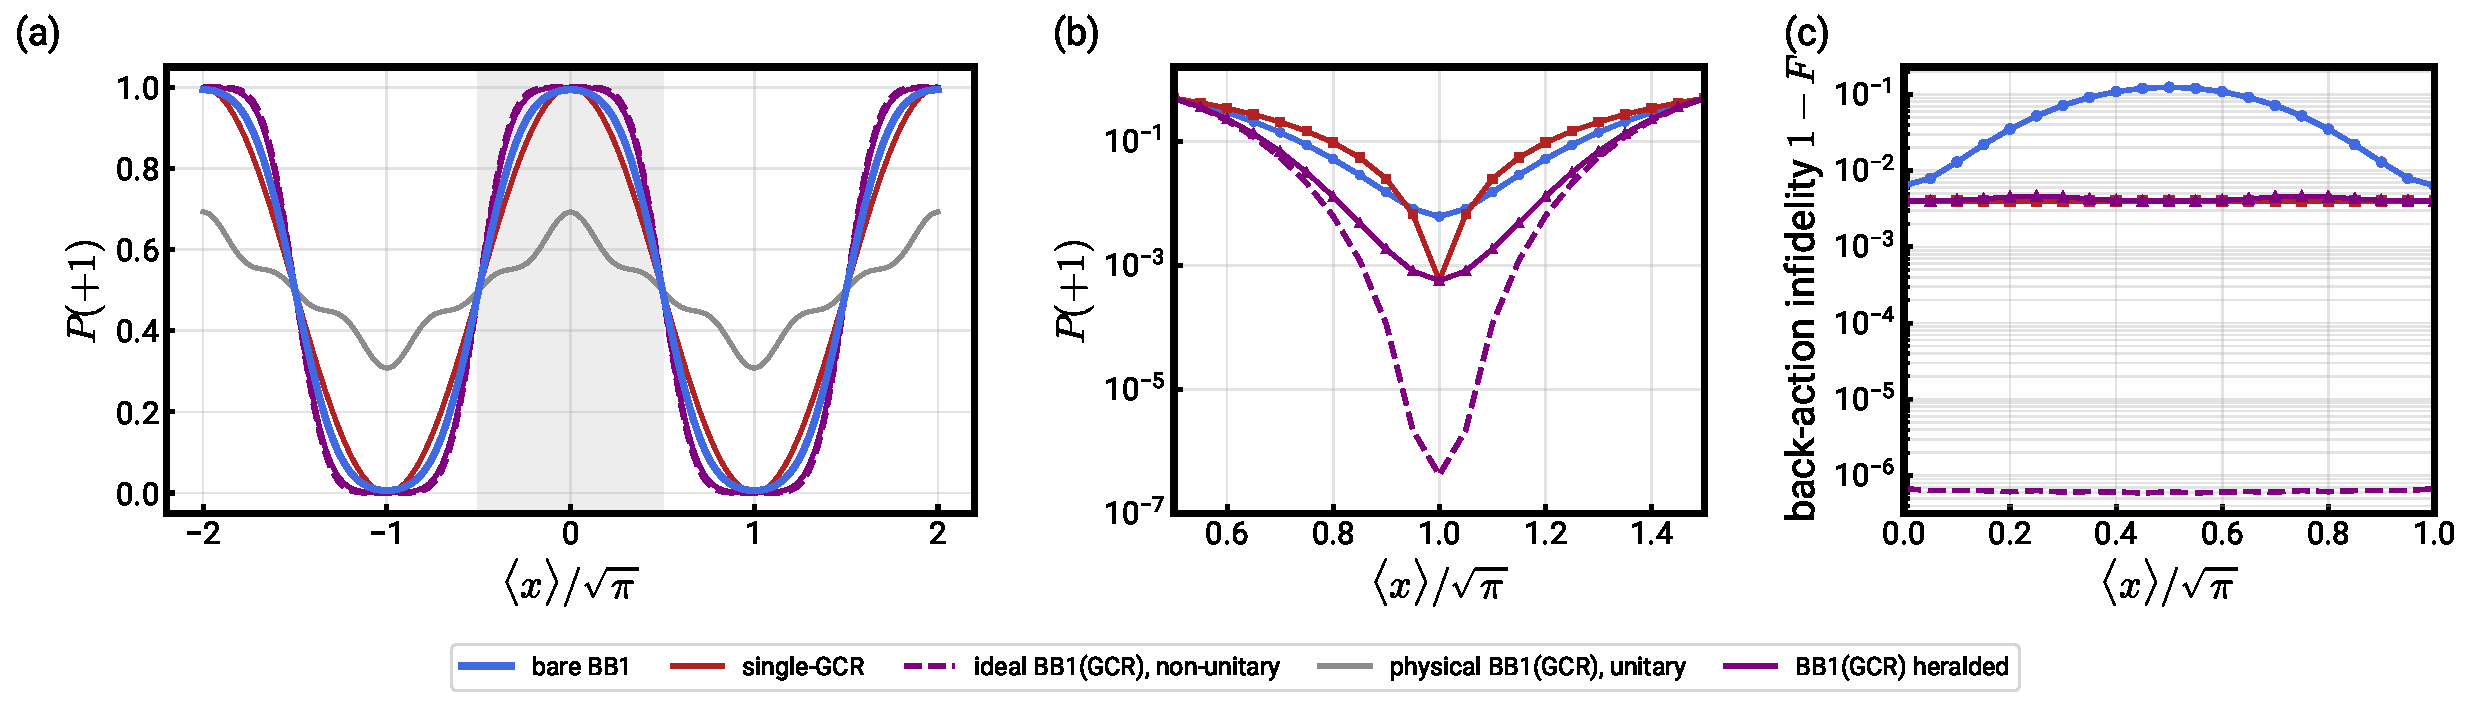
\includegraphics[width=\textwidth]{Supp_Figures/BB1_GCR_fixes.pdf}
\caption{\textbf{(a)} full-range readout: bare (blue), ideal non-unitary (red dashed), and the
unitary split fix $K=1\ldots48$ (green), which only sharpens up to bare. \textbf{(b)} $P(-1)$ near
$\langle x\rangle=0$ (log): the unitary curves plateau at bare near $K{\approx}8$ and never reach
the ideal. \textbf{(c)} heralded non-unitary fix: success vs post-selected error; the
subspace-tailored block-encoding (purple) reaches the ideal at $\sim7\%$, vs $\sim10^{-4}$ for the
global bound (gray).}
\label{fig:main}
\end{figure}

\section{Summary}
The ideal BB1(GCR) readout is genuinely excellent, but its advantage lives entirely in a
\emph{non-unitary} pre-correction. Deterministically, no unitary sequence can beat plain bare BB1:
pulse-splitting (in any of the three schemes tested) plateaus at bare and then degrades, and
amplitude re-optimization does nothing. The only way to recover the ideal readout is to realize
the non-unitary correction \emph{probabilistically}, via an ancilla-heralded block-encoding; with
a low-energy-subspace-tailored encoding this is practical for a repeatable readout (full ideal at
$\sim7\%$ success, $10\times$ over bare at $\sim36\%$). For a deterministic gate, however, BB1(GCR)
offers no advantage over the much shorter bare BB1, and its eight conditional displacements make it
unfavourable for noise --- so it is not pursued as a deterministic primitive.

\end{document}
